%
%
\begin{tikzpicture}[font=\small]
    \tikzstyle{image} = [anchor=center, inner sep=0, outer sep=0, node distance = 0 and 0]
    \pgfplotsset{colormap={cooltowarm_extended}{
    rgb=(0.12548999999999999, 0, 0.38039200000000001)
    rgb=(0.11372500000000001, 0.023529399999999999, 0.45097999999999999)
    rgb=(0.105882, 0.050980400000000002, 0.50980400000000003)
    rgb=(0.039215699999999999, 0.039215699999999999, 0.56078399999999995)
    rgb=(0.031372499999999998, 0.098039200000000007, 0.59999999999999998)
    rgb=(0.043137300000000003, 0.16470599999999999, 0.63921600000000001)
    rgb=(0.054901999999999999, 0.24313699999999999, 0.67843100000000001)
    rgb=(0.054901999999999999, 0.31764700000000001, 0.70980399999999999)
    rgb=(0.050980400000000002, 0.39607799999999999, 0.74117599999999995)
    rgb=(0.039215699999999999, 0.466667, 0.76862699999999995)
    rgb=(0.031372499999999998, 0.53725500000000004, 0.78823500000000002)
    rgb=(0.031372499999999998, 0.61568599999999996, 0.81176499999999996)
    rgb=(0.023529399999999999, 0.70980399999999999, 0.83137300000000003)
    rgb=(0.050980400000000002, 0.80000000000000004, 0.85097999999999996)
    rgb=(0.070588200000000004, 0.85490200000000005, 0.87058800000000003)
    rgb=(0.26274500000000001, 0.90196100000000001, 0.86274499999999998)
    rgb=(0.42352899999999999, 0.94117600000000001, 0.87451000000000001)
    rgb=(0.57254899999999997, 0.96470599999999995, 0.83529399999999998)
    rgb=(0.65882399999999997, 0.98039200000000004, 0.84313700000000003)
    rgb=(0.764706, 0.98039200000000004, 0.86666699999999997)
    rgb=(0.82745100000000005, 0.98039200000000004, 0.88627500000000003)
    rgb=(0.91372500000000001, 0.98823499999999997, 0.93725499999999995)
    rgb=(1, 1, 1)
    rgb=(0.98823499999999997, 0.98039200000000004, 0.87058800000000003)
    rgb=(0.99215699999999996, 0.96470599999999995, 0.71372500000000005)
    rgb=(0.98823499999999997, 0.95686300000000002, 0.64313699999999996)
    rgb=(0.98039200000000004, 0.91764699999999999, 0.50980400000000003)
    rgb=(0.96862700000000002, 0.87451000000000001, 0.40784300000000001)
    rgb=(0.94901999999999997, 0.82352899999999996, 0.32156899999999999)
    rgb=(0.92941200000000002, 0.77647100000000002, 0.27843099999999998)
    rgb=(0.90980399999999995, 0.71764700000000003, 0.235294)
    rgb=(0.89019599999999999, 0.65882399999999997, 0.196078)
    rgb=(0.87843099999999996, 0.61960800000000005, 0.168627)
    rgb=(0.87058800000000003, 0.54901999999999995, 0.156863)
    rgb=(0.85097999999999996, 0.47450999999999999, 0.145098)
    rgb=(0.83137300000000003, 0.41176499999999999, 0.13333300000000001)
    rgb=(0.81176499999999996, 0.34509800000000002, 0.11372500000000001)
    rgb=(0.78823500000000002, 0.26666699999999999, 0.094117599999999996)
    rgb=(0.74117599999999995, 0.18431400000000001, 0.074509800000000001)
    rgb=(0.69019600000000003, 0.12548999999999999, 0.062745099999999998)
    rgb=(0.61960800000000005, 0.062745099999999998, 0.043137300000000003)
    rgb=(0.54901999999999995, 0.027451, 0.070588200000000004)
    rgb=(0.47058800000000001, 0.0156863, 0.090196100000000001)
    rgb=(0.40000000000000002, 0.0039215700000000001, 0.101961)
    rgb=(0.34902, 0, 0.129412)
}}
    \pgfplotsset{colormap={green_purple}{
    rgb=(0.23137254901960799, 0, 0.34509803921568599)
    rgb=(0.337254901960784, 0, 0.44313725490196099)
    rgb=(0.44705882352941201, 0, 0.54117647058823504)
    rgb=(0.60392156862745106, 0.015686274509803901, 0.65098039215686299)
    rgb=(0.76470588235294101, 0.035294117647058802, 0.76470588235294101)
    rgb=(0.88235294117647101, 0.21568627450980399, 0.82352941176470595)
    rgb=(1, 0.50980392156862697, 0.90588235294117603)
    rgb=(1, 0.76470588235294101, 0.95294117647058796)
    rgb=(1, 1, 1)
    rgb=(0.85882352941176499, 0.94901960784313699, 0.49803921568627502)
    rgb=(0.71764705882352897, 0.90196078431372595, 0)
    rgb=(0.54117647058823504, 0.82745098039215703, 0)
    rgb=(0.36470588235294099, 0.752941176470588, 0)
    rgb=(0.25490196078431399, 0.64313725490196105, 0)
    rgb=(0.149019607843137, 0.53725490196078396, 0)
    rgb=(0.074509803921568599, 0.40000000000000002, 0.023529411764705899)
    rgb=(0, 0.26300000000000001, 0.050999999999999997)
}}
    \node[image] (image1)
    {
        \begin{tikzpicture}
            \node[image] (base) at (0,0) {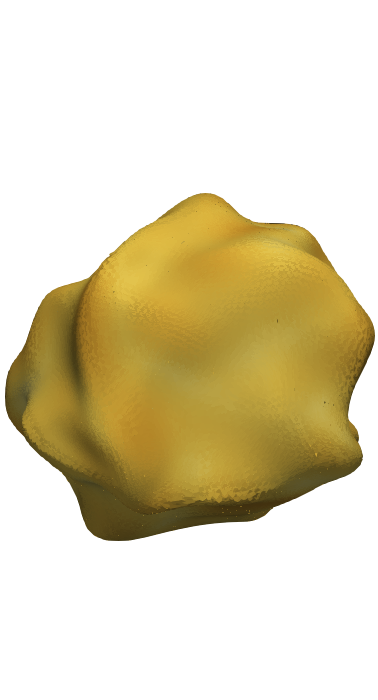
\includegraphics[height=0.2585\figurewidth]{figures/spherical_time_1_02e-4}};%
            \clip (base.south west) -- (base.north west) -- (base.north east) -- (base.south east) -- cycle;
            \clip (-2.0, -3.5) -- (2.0, 3.5) -- (4.0, 3.5) -- (4.0, -3.5)  -- cycle;
            \node[image] at (0,0) {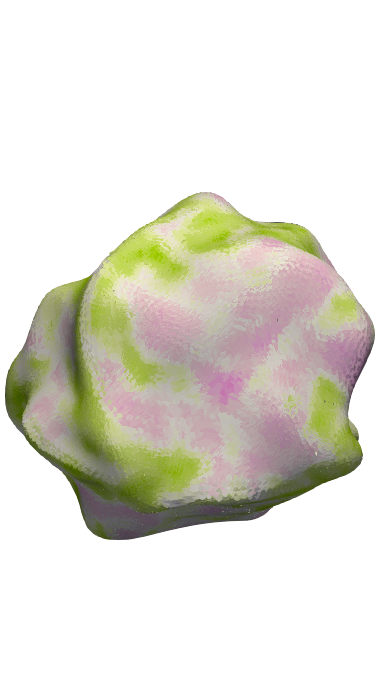
\includegraphics[height=0.2585\figurewidth]{figures/spherical_time_1_02e-4_density_factor}};%
        \end{tikzpicture}
    };
    \node[anchor=north, align=left] at (image1.south) {$t = \SI{1.02e-4}{\second}$ \\ $N=\num{50}\si{\kilo}$};
    \node[image, right=of image1] (image2)
    {
        \begin{tikzpicture}
            \node[image] (base) {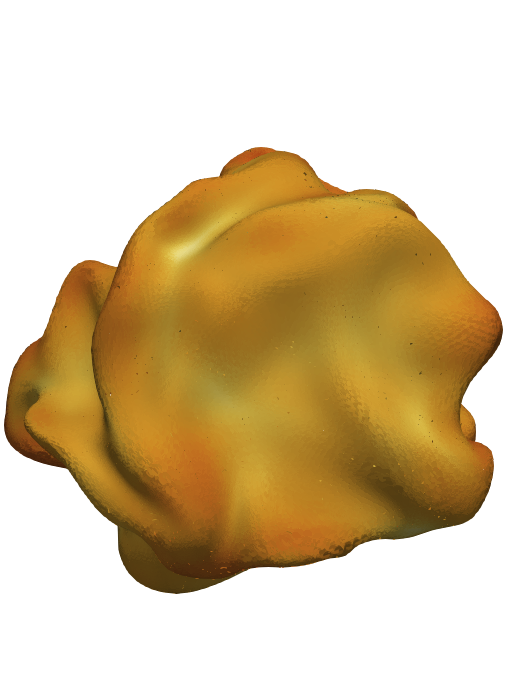
\includegraphics[height=0.2585\figurewidth]{figures/spherical_time_1_7e-4}};%
            \clip (base.south west) -- (base.north west) -- (base.north east) -- (base.south east) -- cycle;
            \clip (-2.0, -3.5) -- (2.0, 3.5) -- (4.0, 3.5) -- (4.0, -3.5)  -- cycle;
            \node[image] {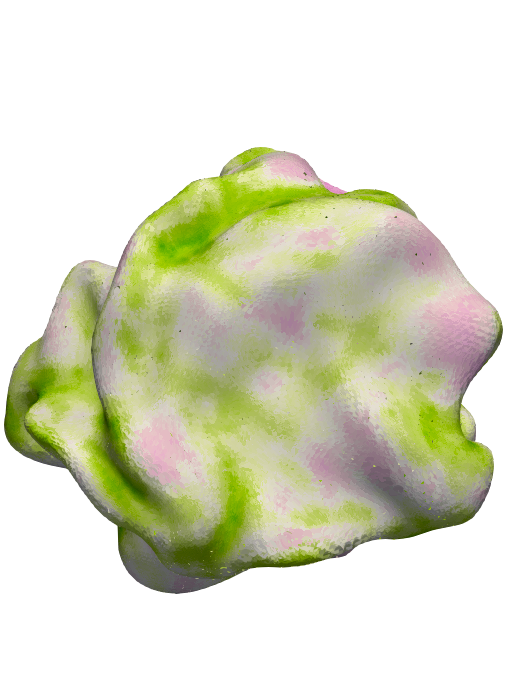
\includegraphics[height=0.2585\figurewidth]{figures/spherical_time_1_7e-4_density_factor}};%
        \end{tikzpicture}
    };
    \node[anchor=north, align=left] at (image2.south) {$t = \SI{1.7e-4}{\second}$ \\ $N=\num{140}\si{\kilo}$};
    \node[image, right=of image2] (image3)
    {
        \begin{tikzpicture}
            \node[image] (base) {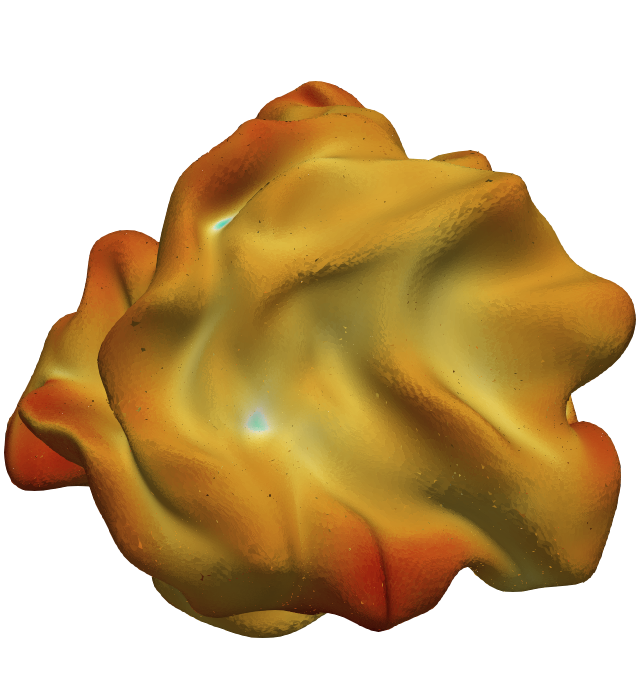
\includegraphics[height=0.2585\figurewidth]{figures/spherical_time_2_4e-4}};%
            \clip (base.south west) -- (base.north west) -- (base.north east) -- (base.south east) -- cycle;
            \clip (-2.0, -3.5) -- (2.0, 3.5) -- (4.0, 3.5) -- (4.0, -3.5)  -- cycle;
            \node[image] {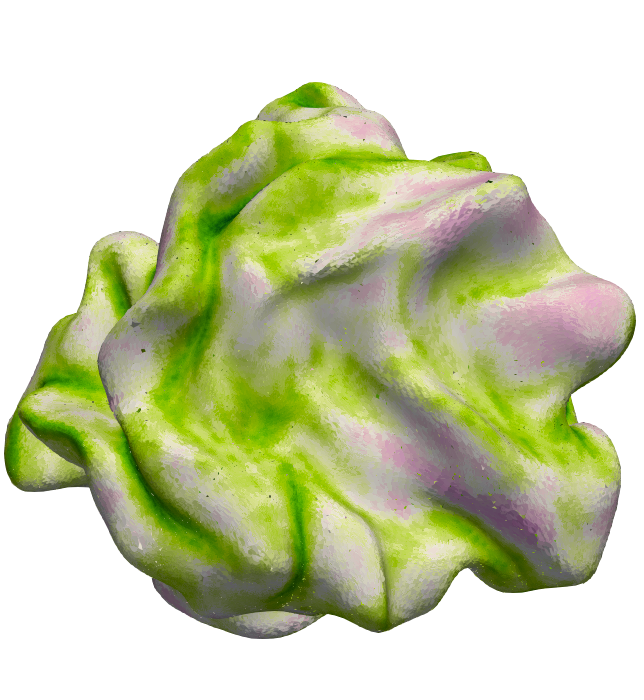
\includegraphics[height=0.2585\figurewidth]{figures/spherical_time_2_4e-4_density_factor}};%
        \end{tikzpicture}
    };
    \node[anchor=north, align=left] at (image3.south) {$t = \SI{2.4e-4}{\second}$ \\ $N=\num{400}\si{\kilo}$};
    \node[image, right=of image3] (image4)
    {
        \begin{tikzpicture}
            \node[image] (base) {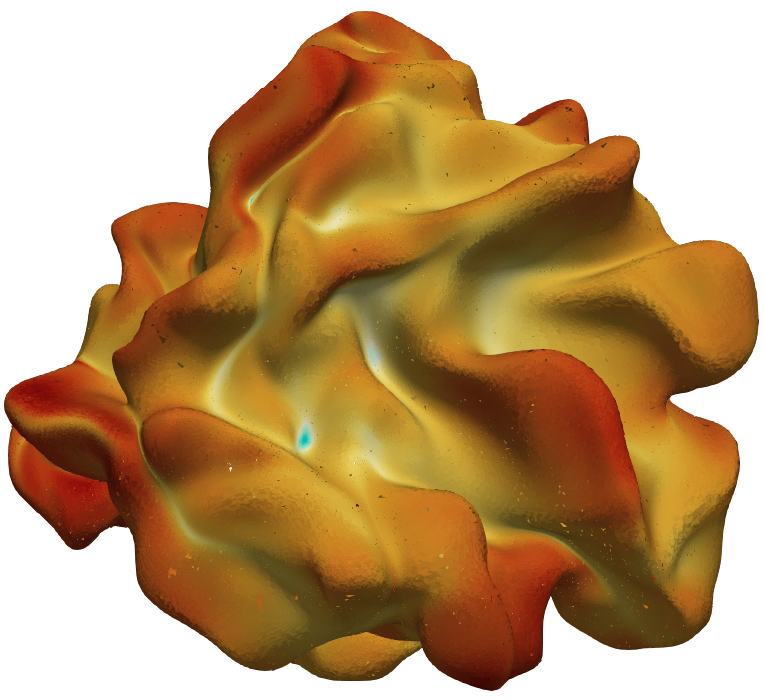
\includegraphics[height=0.2585\figurewidth]{figures/spherical_time_3e-4}};%
            \clip (base.south west) -- (base.north west) -- (base.north east) -- (base.south east) -- cycle;
            \clip (-2.0, -3.5) -- (2.0, 3.5) -- (4.0, 3.5) -- (4.0, -3.5)  -- cycle;
            \node[image] {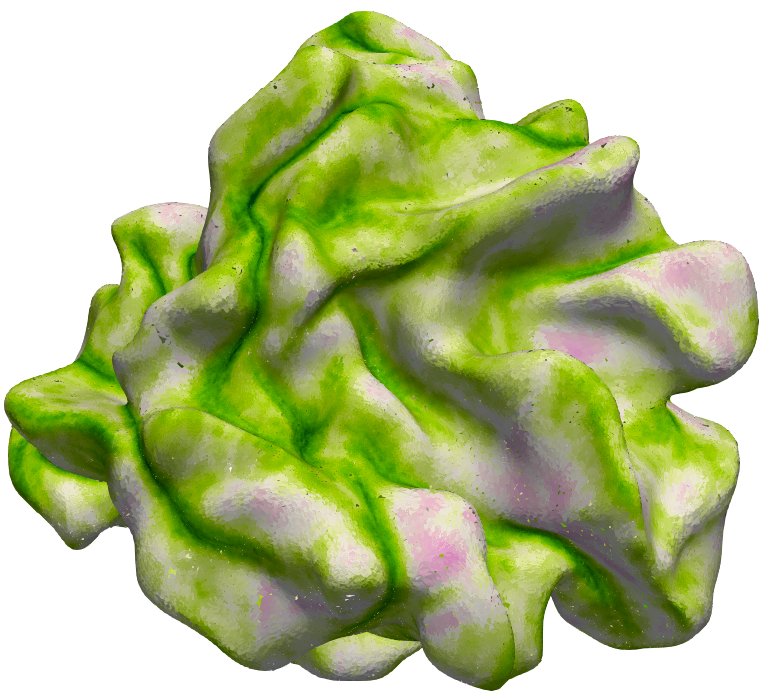
\includegraphics[height=0.2585\figurewidth]{figures/spherical_time_3e-4_density_factor}};%
        \end{tikzpicture}
    };
    \node[anchor=north, align=left] at (image4.south) {$t = \SI{3.1e-4}{\second}$ \\ $N=\num{870}\si{\kilo}$};

    \node (bbnw) at ($(image1.north west) + (-1.25, 0.4)$) {};
    \node (bbse) at ($(image4.south east) + (1.35, -0.45)$) {};

    \clip (bbnw) rectangle (bbse);

    \node[anchor=east, xshift=-0.1cm] at (image1.west){
        \begin{axis}[
        scale only axis,
        height=4.5cm,
        hide axis,
        domain=1.5:1.5,
        colorbar,
        colorbar/width=0.25cm,
        colormap name={cooltowarm_extended},
        point meta min=-1.5, point meta max=1.5,
        colorbar style={
            title=$c$,
            scaled ticks=false,
            yticklabel pos=left,
            ytick={-1, 0, 1},
            yticklabels={$10^{-1}$, $10^{\,0}$, $10^{\,1}$},
            % extra y ticks ={0.3, 0.4771212, 0.60206, 0.69897, 0.778151, 0.845098, 0.90309, 0.954242, 1.3, 1.4771212,
            %                 -0.3, -0.4771212, -0.60206, -0.69897, -0.778151, -0.845098, -0.90309, -0.954242, -1.3, -1.4771212},
            % extra y tick labels=\empty
        }]
      \end{axis}
    };
    \node[anchor=west, xshift=-0.5cm] at (image4.east){
        \begin{axis}[
        scale only axis,
        height=4.5cm,
        hide axis,
        domain=-2.5:2.5,
        colorbar,
        colorbar/width=0.25cm,
        colormap name={green_purple},
        point meta min=-2.5, point meta max=2.5,
        colorbar style={
            title=$d$,
            scaled ticks=false,
            yticklabel pos=right,
            ytick={-2, -1, 0, 1, 2},
            yticklabels={$10^{-2}$, $10^{-1}$, $10^{\,0}$, $10^{\,1}$, $10^{\,2}$},
            % extra y ticks ={1, 1.3, 1.4771212, 1.60206, 1.69897, 1.778151, 1.845098, 1.90309, 1.954242,
            %                 -1, -1.3, -1.4771212, -1.60206, -1.69897, -1.778151, -1.845098, -1.90309, -1.954242},
            % extra y tick labels=\empty
        }]
      \end{axis}
    };
\end{tikzpicture}%
